\section{Introdu��o}

Este projeto tem como objetivo construir um compilador de um subconjunto de OCL
(Object Constraint Language) para a linguagem Go. O subconjunto referido se
preocupa em tratar as restri��es que definem o corpo de opera��es de consulta,
utilizando a \textit{keyword} \textbf{body}. Para reduzir o escopo de OCL foram
utilizadas as gram�ticas:  \verb![Kleppe]!,
(\href{http://www.yancy.org/school/lehigh/phd/links/ocl-grammar-01b.pdf}{\texttt{http://www.yancy.org/school/lehigh/phd/links/ocl-grammar-01b.pdf}})
e a \verb![Especifica��o OCL]!.

Na primeira etapa do projeto foram constru�das as fases de An�lise L�xica e An�lise Sint�tica. Para construir o Analisador L�xico e o Analisador Sint�tico foram utilizadas as ferramentas JFlex e JCup respectivamente. 

Um esbo�o da arquitetura do ''Compilador de OCL para Go'' � apresentando na
imagem abaixo. Constru�do em Java, o compilador possui tr�s pacotes:
\verb!analise_lexica!, \verb!analise_sintatica! e \verb!util!.

\begin{figure}[h!]
	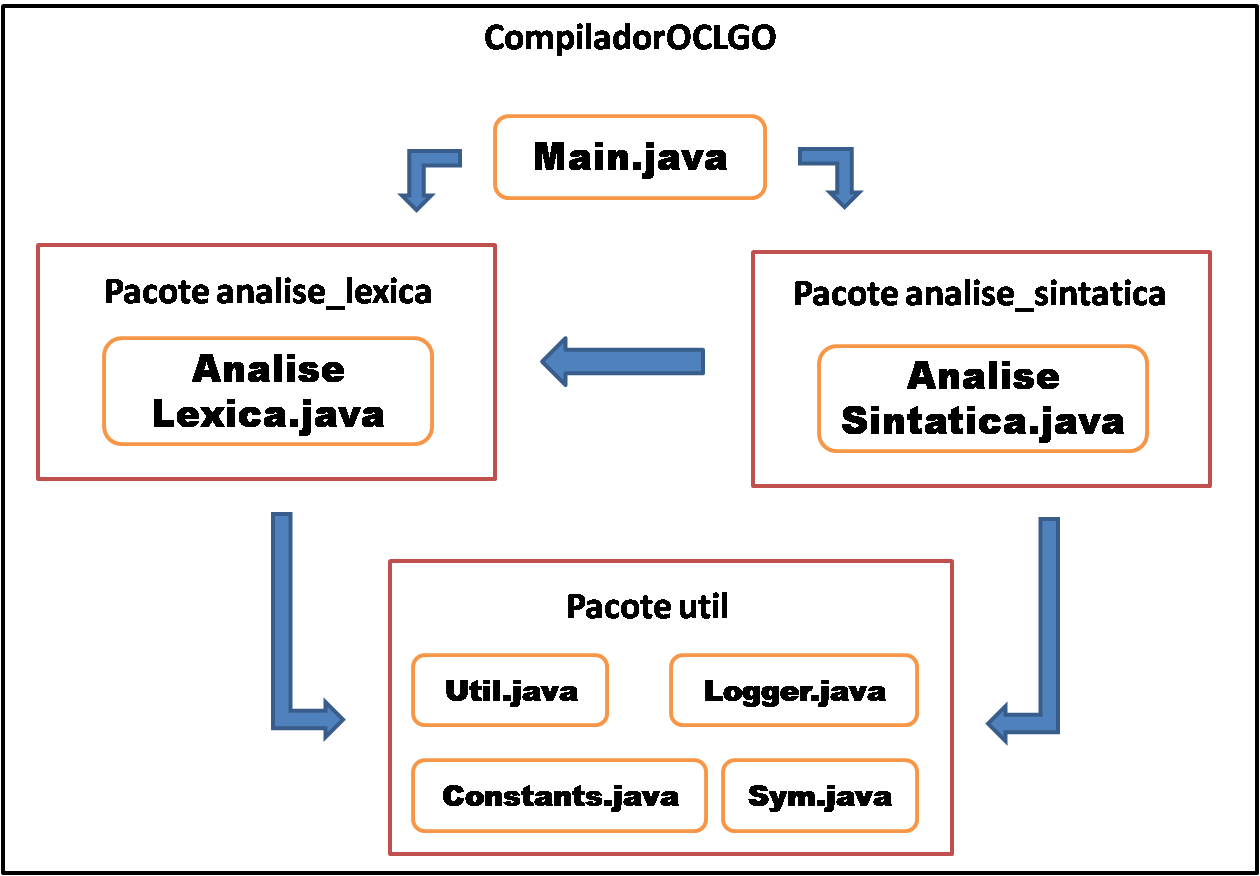
\includegraphics[scale=0.5]{imagens/compilador.png}
	\caption {Compilador OCL para Go.}
\end{figure}

O pacote util � formado pelas classes:
\begin{itemize}
  \item Util.java - possui opera��es auxiliares para tratar como os tokens ser�o
  apresentados para o usu�rio;
  \item Logger.java - possui opera��es que tratam as mensagens de erros da
  analise l�xica;
  \item Constants.java - possui constantes que auxiliam na apresenta��o dos
  tokens para o usu�rio;
  \item Sym.java - possui as constantes que representam os tokens.
\end{itemize}

O analisador l�xico (representado pela classe \textbf{AnaliseLexica.java})
utiliza o pacote util para auxiliar no reconhecimento dos tokens. O analisador sint�tico
(representado pela classe \textbf{AnaliseSintatica.java}) utiliza as classes do
pacote Util e do pacote \verb!analise_lexica!, mais especificamente a classe
AnaliseLexica.java, para realizar a an�lise sint�tica.
 